\chapter{State of the art}

\section{Intraoperative ultrasound}
\textcolor{green}{Start with why US is used, then describe how it works and the limitations. from there you should have a nice transition to navigation}
In
liver surgeries an intraoperative ultrasound device is used for intraoperative planning and
navigation inside the liver. It is used to locate tumors that are not
visible on the liver surface and to estimate their sizes from the ultrasound image. Figure \ref{fig:liverUS} shows an example of an
ultrasound image of the liver and its corresponding position in the 3D liver
model.

\begin{figure}[H]
  \centering
 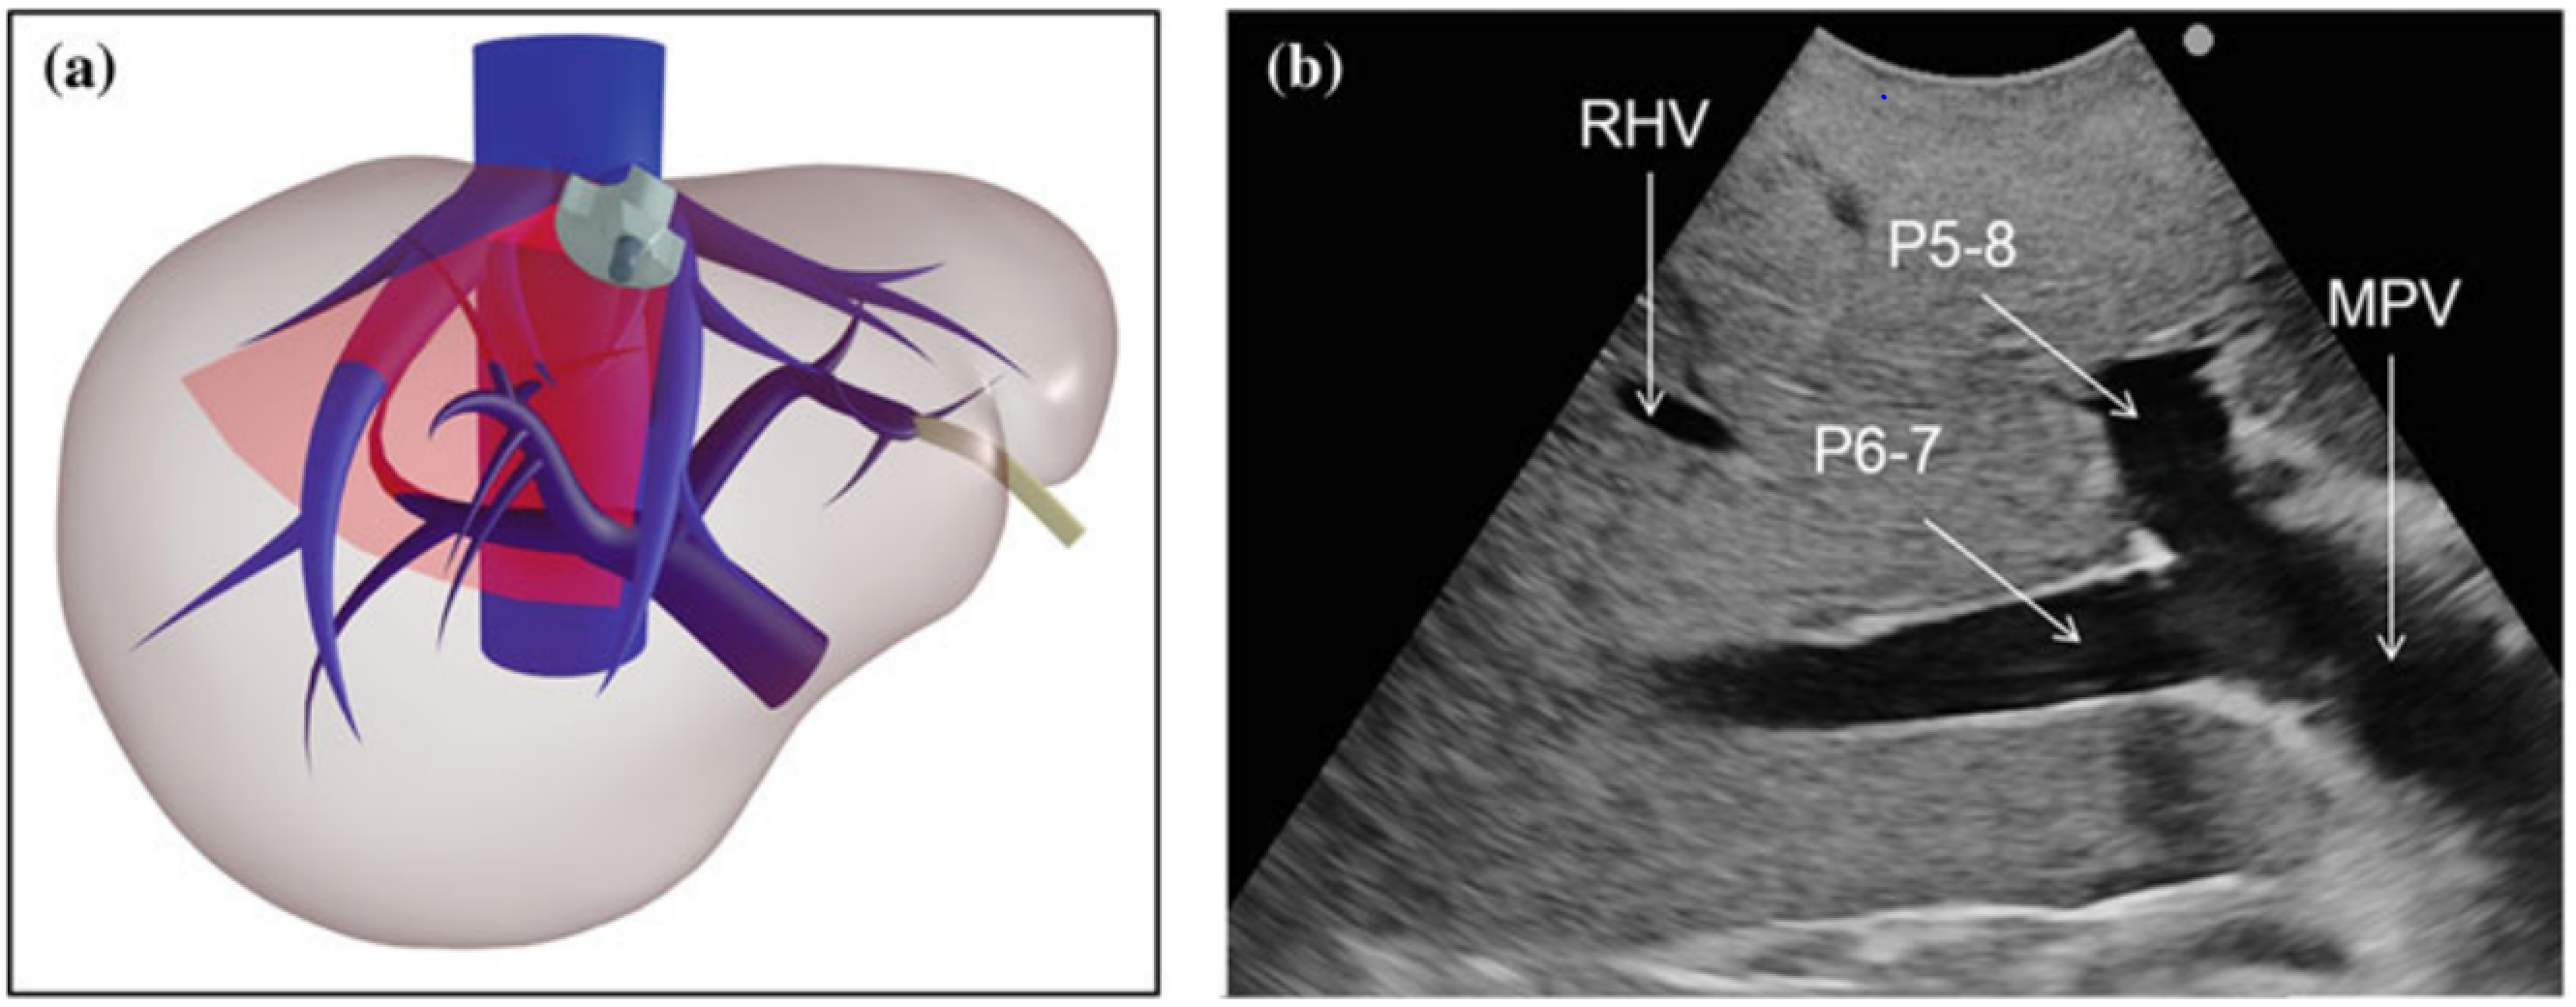
\includegraphics[width=\textwidth]{liverUS}
 \caption{ Left (a) ultrasound image plane in the liver. Right (b) intraoperative
   ultrasound image. One can see the right hepatic vein (RHV), the portal branch
   to segments 5 and 8 (P5-8) and the portal branch to segments 6 and 7 (P6-7) \cite{torzilli2014ultrasound}}
  \label{fig:liverUS}
\end{figure}

Ultrasound imaging works by the \textit{pulse-echo} principle. A short
ultrasound pulse is emitted from a transducer. The sound waves get
transmitted and reflected differently by different tissues. The reflected
 waves travel back into the transducer and are converted into an electrical
signal. After post-processing these signals become ultrasound images. 
The ultrasound measures the mechanical properties of the tissue. The tissues
have different acoustic impedance, which is the product of tissue density and
ultrasound speed in travelling through the tissue. The resolution of the
ultrasound images depends on the frequency of the ultrasonic waves. High
frequencies lead to higher resolution but lower penetration depth into the tissue because the
absorption of the sound energy increases with frequency too. Therefore the
useability to see deep structures is limited \cite{torzilli2014ultrasound}. 

In liver surgeries ultrasound is an important and established instrument.
Intraoperatively, the ultrasound is used on the liver surface directly,
therefore the penetration depth of the
ultrasound is optimal to represent the inner structures of the liver.
Registration methods based on 3D ultrasound reconstructed liver vessels 
exist but are not used in practice frequently \cite{lange2003vessel}. Ultrasound
is not harmful to health and therefore, can
be used as often as desired to navigate during a surgery.
% it is  
% Intraoperatively surgeons use ultrasound to localize the tumor as it gives
% advantages of reduced surgical time, complexity and radiation dosage.

\section{Navigation for liver resections}
\label{sec:navigationForLiverResections}
\textcolor{green}{first, why is navigation needed, then how does it generally work
  1) preoperative model or surgical plan 2) tracking 3) registration 4)
  navigation visualization etc. then challenges especially in liver surgery and limitations}
It is a difficult task for inexperienced surgeons to orientate themselves within the liver during an operation.
From the outside of the liver it is not visible where the blood vessels are which they do not want to hurt.
Navigation can help surgeons to orient themselves precisely in organs during
operations.

% The actual intervention in computer assisted surgeries (CAS) is defined as
% surgical navigation.
A navigated operation differs in a few points from a non-navigated operation.
Because every patient's liver is different, a new 3D model of the liver has to
be created before surgery. This models are created from pre-operative 3D
computer tomography (CT) scan of the liver. Then, using this model, a surgical plan is made.
In contrast to a regular operation, a navigation system is located in the
operating theatre and the surgical instruments can be tracked by it. Therefore special instruments are used. These
instruments have the ability to be tracked by the naviagation system. Depending
on the tracking technology used by the navigation system, the tools are different.
In order to also track the liver, the created model is registered to the anatomy
of the patient. Finally the orientation and position
of the instruments in relation to the patient's anatomy is visualized on a
monitor in the operating room. The surgeon can see what he does on the
monitor and uses the system to navigate the location and position of its
instruments. This is specialy then useful when the tip of the instrument is not
actually visible for the suergeon.

The achieved
navigation accuracy with such a system was 4.5 mm $\pm$3.6 mm averaged over nine surgeries \cite{peterhans2011navigation}.
Current research tries to compensate for deformations of the liver after the CT
scan to the actual shape of the liver \cite{clements2017deformation}
\cite{clements2015validation}. 
\subsection{Creation of preoperative 3D-models}
Several steps are necessary to create a preoperative model. First the 
CT scan is done. This leads to representations of the liver on several 2D images parallel
to each other, filling a square volume with voxels. From this data the liver and
its inner structures are manually segmented and merged to a 3D model (Figure \ref{fig:MeVisExample}). This is very
time consuming and therefore expensive \cite{numminen2005preoperative}.
Nevertheless the resulting models are very detailed and accurate.
\begin{figure}[H]
  \centering
 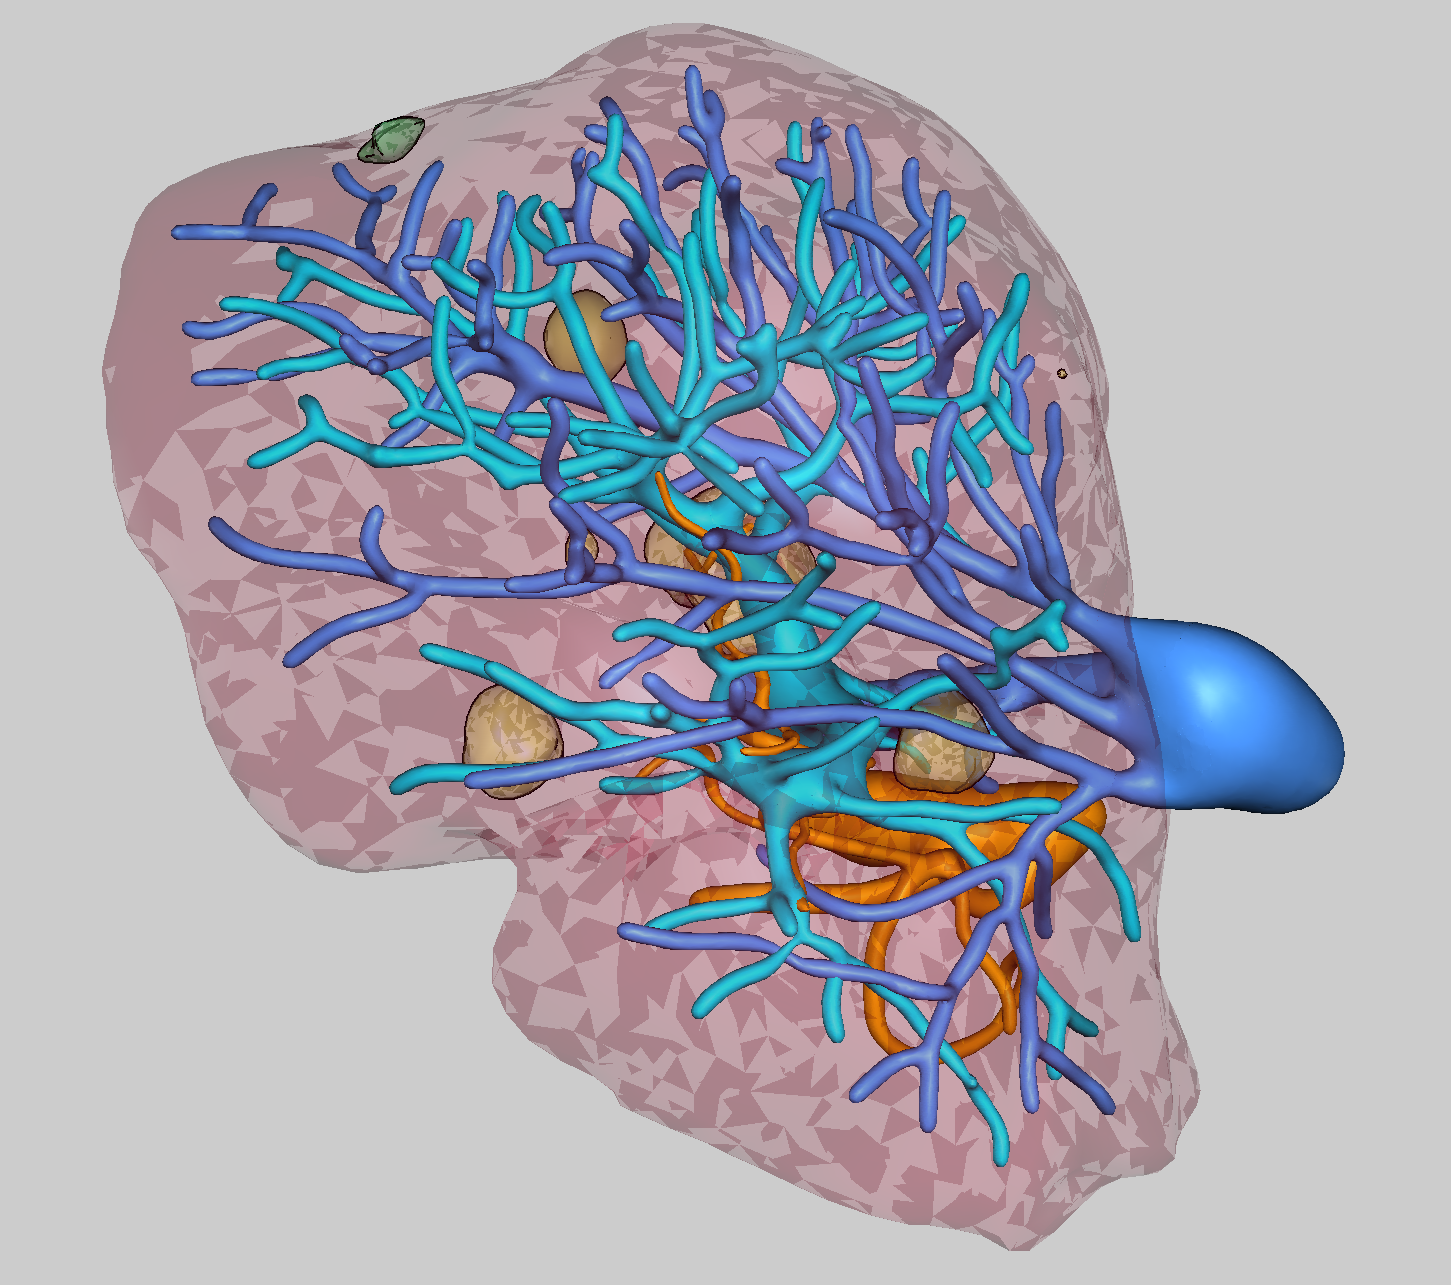
\includegraphics[width=0.6\textwidth]{MeVisExample}
 \caption{Example of a preoperative 3D model created by MeVis}%DK patient
  \label{fig:MeVisExample}
\end{figure}

\subsection{Registration methods}
Patient registration is a concept to correlate the reference coordinate system
of a virtual 3D data set with that of a patient. First, the 3D data set has to
be gathered. This is often done by CT or MRI scan of the patients anatomy to be
operated on. Secondly, finding of the transformation between the patient's
reference coordinate system and the virtual data set. During the surgery the patient is similarly
tracked as the instruments (see section \ref{sec:navigationForLiverResections}).
In this way, the patient has his own coordinate system. From here many different
methods exist to align the virtal data to the real anatomy.
Discrete landmarks, surface scans and
volumetric sonography scans are just a few of the approaches that can be
used to achieve precise alignment of the data with the
surgical site \cite{banz2016intraoperative}. 

\subsubsection{Surface registration}
\textcolor{red}{Start with why Surface registration is used, then describe how it works and the limitations. from there you should have a nice transition to navigation}

Surface registration is registration based on surfaces. It is used and studied
for several years in all kinds of fields \cite{ramos2015review}. Especially in
the field of medical technology, a lot of research is being done in the
direction of contactless registration. Intraoperatively, different camera technologies which lead
to depth images are used to sample the surface of an organ. Often used imaging systems are stereo cameras
\cite{furukawa2010accurate}, structured light \cite{salvi2004pattern} and
laser range scanners \cite{cash2003incorporation}. From these intraoperatively
created data sets, surfaces are reconstructed and then used for registration. To
find the mapping between the surfaces, mostly different variants of the iterative
closest point (ICP) \cite{besl1992method} algorithm are used. 

These surface based methods are limited to structures on the outer part of the
organ because. 
Researchers try to compensate for intraoperative soft-tissue deformations
\cite{cash2005compensating}\cite{dagon2008real}.
\subsection{Tracking modalities}
To track surgical instruments and patient's anatomy (define the position and
orientation in real time) during naviagated surgery a tracking system is needed.
Tracking can be done by different technologies. The most used tracking
modality is optical tracking. 

\subsubsection{Optical tracking}
Optical tracking is the most used tracking modality in naviagated liver
surgeries. Passive markers (spherical, retro-reflective that reflect infrared
light) or active markers (infrared-emitting markers that are activated by an
electrical signal) \cite{wiles2004accuracy} are attached to the objects that
need to be tracked. A tracking camera is then emitting infrared light by illuminators
on the position sensor (only for passive markers). The position sensor
determines the position and orientation of the tracked instruments based on the
information it receives from those markers \cite{noauthor_polaris_nodate}.  

\section{Surface reconstruction from unorganized points}
\textcolor{green}{First, collecting the sample ... These terms should match the titles below
Both other chapters, explain first what the process is for, then what methods are available}
A surface reconstruction's goal is to create a surface from sampled points \cite{berger2017survey}. Two
main steps need to be processed. First, acquisition of the data to create a sample. Secondly,
apply a reconstruction algorithm on the sampled points.
\subsection{Data acquisition}
\textcolor{green}{what the process is for, then what methods are available}
In order to reconstruct a surface it is necessary to have some information about
it. Therefore a set of points which lie on or near the unknown surface is acquired first. A
reconstruction algorithm has then to reconstruct the surface from these points.

There exist different methods to collect surface points
\cite{franca20053d}\cite{levoy2000digital}\cite{cui20113d}\cite{chu2002infrared}\cite{dou20153d}.
Optical (non-contact scan) scans are the most popular ones. Specialy laser based
scanners can scan very fast and with a precision in the order of micrometers. Also contact scans exist
\cite{pai2001scanning}. Contact scans can also be very precise (in the order of
micrometers).

In the field of liver surface scanning only a few articles were published  \cite{maier2014comparative} \cite{thompson2015accuracy}. 
They used stereo laparoscopic cameras to sample the surface.
\subsection{Reconstruction algorithms}
\textcolor{green}{ switch explicit and implicit, so you have the same order as in the figure}

\textcolor{green}{what the process is for, then what methods are available}
The problem
surface reconstruction aims to solve is the representation of a surface in 
digital form, from error containing data that has first been scanned in the
real world.

Again, a lot of reconstruction algorithms exist \cite{lim2014surface}, but not
all of them are made to reconstruct from unorganized points. This means
that the point orders, orientations, connections and the topological type of the
surface is not known a priori. Therefore it is necessary that the algorithm does not assume any structure
on the data points \cite{hornung2006robust} \cite{yu1999surface}. The orientations, connections and the topological
type must be inferred from the points. This is a major difficulty of the general surface
reconstruction problem \cite{hoppe1992surface}. In the past few decades, many
algorithms that can solve this problem have been published. Nevertheless it is
still a challanging task that is part of current research \cite{li2018surface}.
The available reconstrction types can be classified into two groups: implicit
volume-based and explicit mesh-based reconstructions.
\begin{figure}[H]
  \centering
 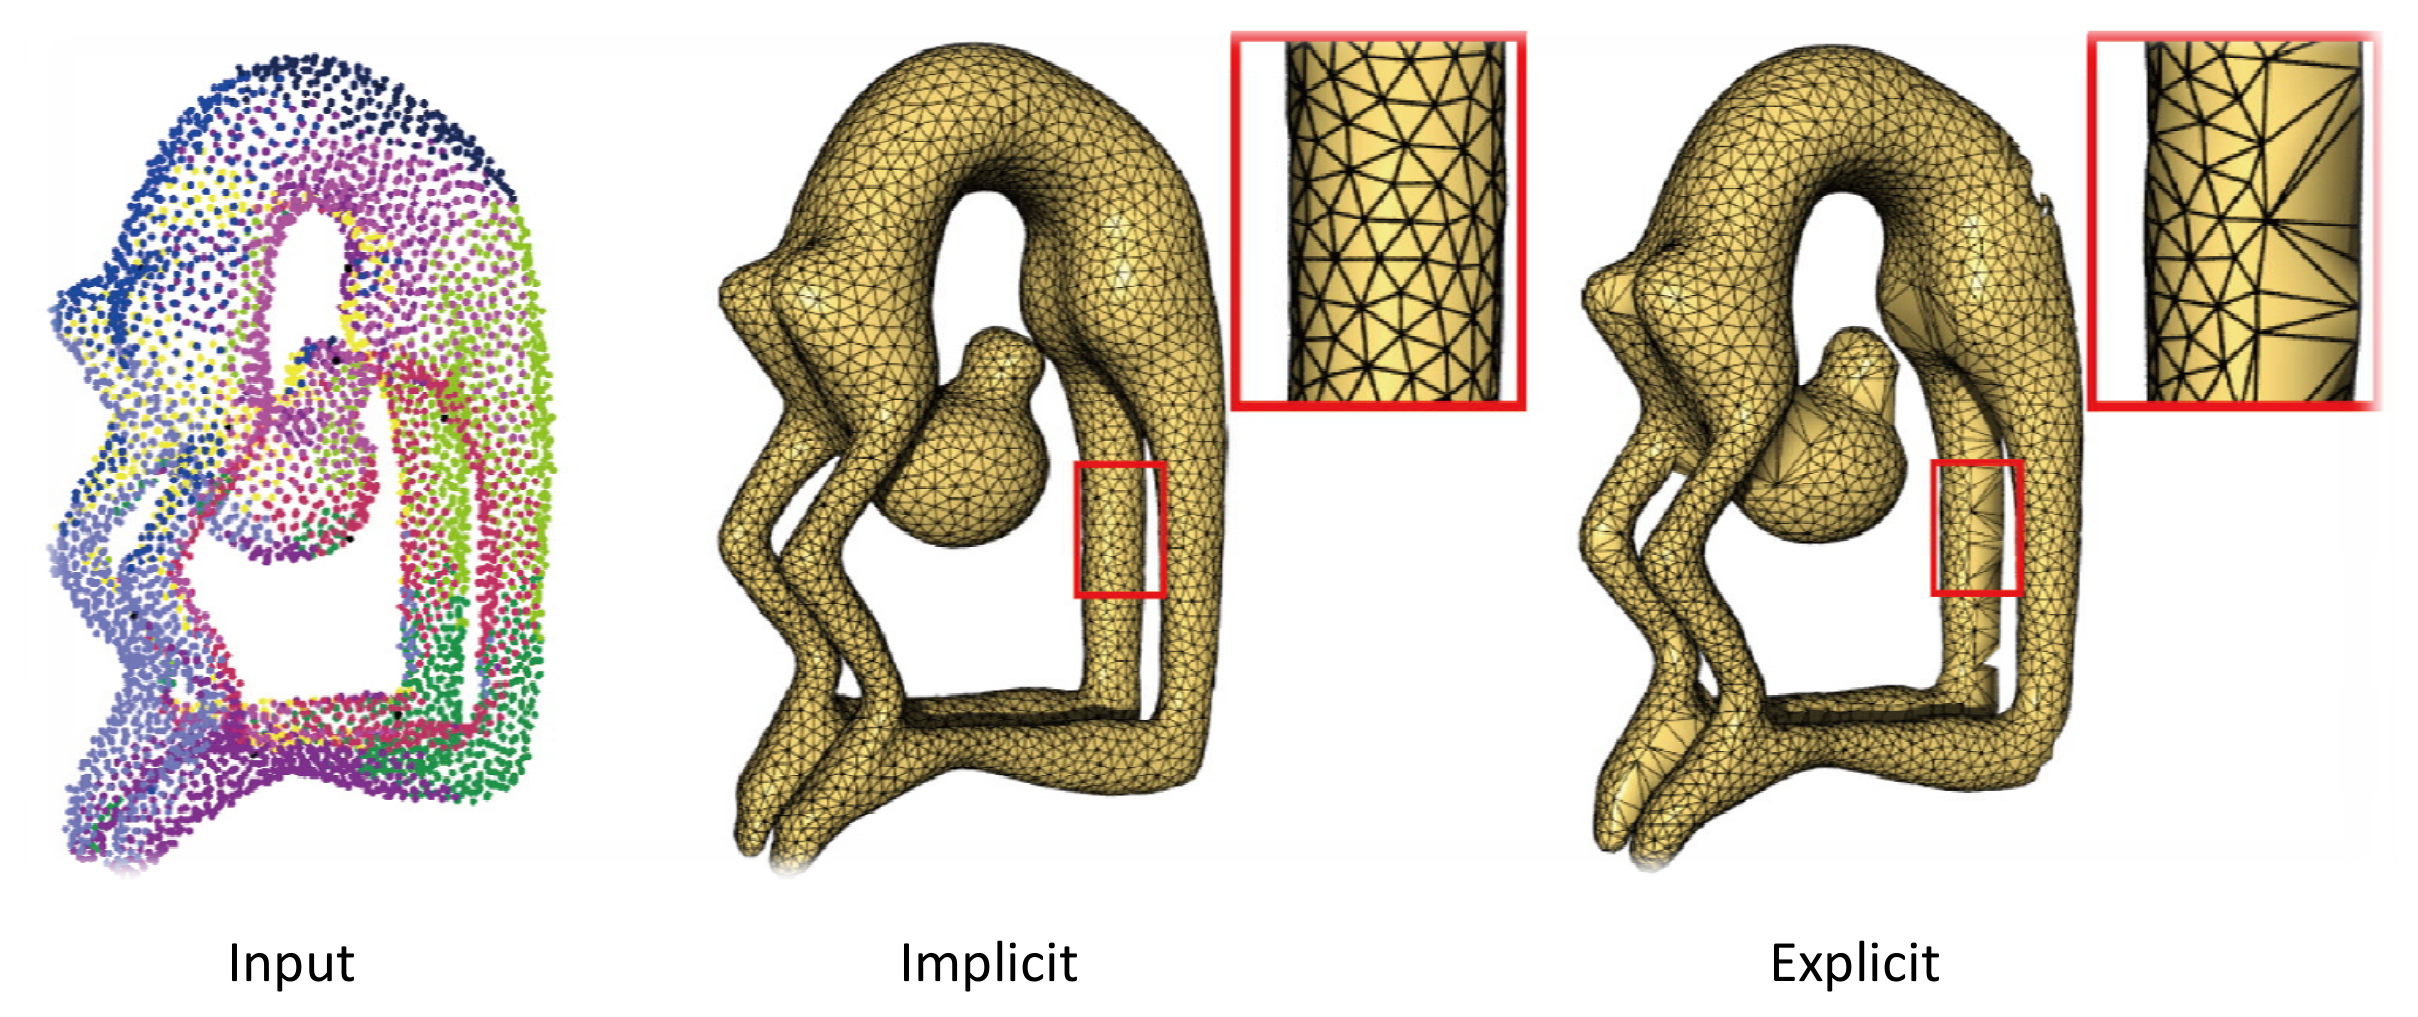
\includegraphics[width=\textwidth]{ImplicitVSExplicit}
 \caption{The difference between implicit and explicit surface reconstructions.
   On the left side is the pointcloud used as input. In the middle the result of an
   implicit reconstruction. On the right side the result of an explicit
   reconstruction \cite{stanfordPP}}
  \label{fig:ImplicitVSExplicit}
\end{figure}
\subsubsection{Implicit volume-based reconstrction}
Implicit volume-based reconstruction techniques construct an implicit
volume-function from the input points. From the iso-surface of the
volume-function a restored surface can then be optained. For these methods it is
not a problem if the surface topology is complex. But most of these methods
suffer from oversmoothing the data and the need of accurate directions of normal
vectors in addition to the unorganized points. 
\subsubsection{Explicit mesh-based reconstrction}
Explicit mesh-based reconstrction methods form a triangular mesh directly from
the unorganized points. These mesh-based reconstructions are precise but they
have problems with noise, complex shapes and especially holes in data.


% \cite{kazhdan2005reconstruction} oriented point set hornung2006robust
% \cite{hornung2006robust} non uniformly sampled point clouds without normal information
% \cite{yu1999surface} NN to reconstruct from unorganized points



% \begin{itemize}
%   \item not tracked laproscopic one shot images stereo with registration
%   \item moved laproscopic tracked endoscope stereo with registration 
% \end{list}

% \cite{hoppe1992surface}

\endinput
%%% Local Variables:
%%% TeX-master: "MscThesis"
%%% End: